\documentclass[crop,tikz]{standalone}% 'crop' is the default for v1.0, before it was 'preview'
\usepackage{tikz,calc,pgfplots}
\usepackage{tikz-3dplot}
\usetikzlibrary{calc}
\usetikzlibrary{calc,patterns,decorations.pathmorphing,decorations.markings}
\usetikzlibrary{shapes.geometric}
\begin{document}


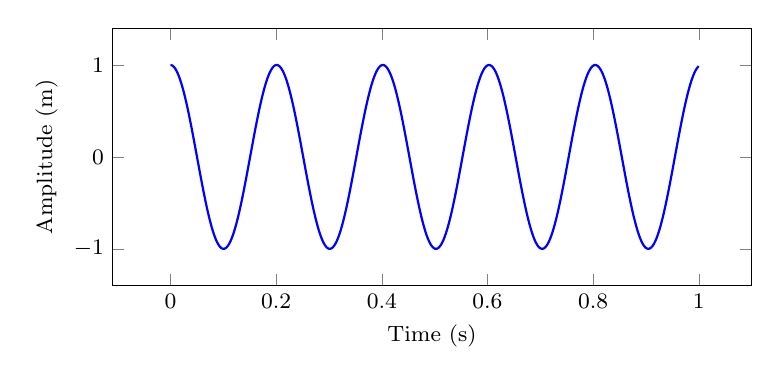
\begin{tikzpicture}[scale=1]
	\footnotesize
	\begin{axis}[
		width=0.8\textwidth,
		height=0.4\textwidth,
		xlabel={Time (s)},
		ylabel = {Amplitude (m)},
		xmax=1.1,
		ymax=1.4,
		ymin=-1.4,  
		samples=500]
		
		\def\wn{5*2*pi};
		\def\xo{1};
		\def\dxo{0};		
		\def\zEta{0.1};
		\def\wdd{sqrt(1-\zEta^2)*\wn};
		\def\Phii{rad(atan(\dxo/(\wdd*\xo)))};
		
		
%		\addplot[gray!50!white, thick, domain=0:1] (x, {sqrt(\xo^2+(\dxo/\wdd)^2) * cos(deg(\wdd*x- \Phii))});
%		\addplot[red,dashed, thick, domain=0:1] (x, {sqrt(\xo^2+(\dxo/\wdd)^2) * exp(-\zEta*\wn*x)});
%		\addplot[red,dashed, thick, domain=0:1] (x, {-sqrt(\xo^2+(\dxo/\wdd)^2) * exp(-\zEta*\wn*x)});	
		\addplot[blue, thick, domain=0:1] (x, {sqrt(\xo^2+(\dxo/\wdd)^2) * cos(deg(\wdd*x- \Phii)) * exp(-0*\wn*x)});
		
	\end{axis}
	
	%	
	%	\begin{axis}[
		%		width=0.9\textwidth,
		%		height=0.4\textwidth,
		%		%axis y line*=right,
		%		%xmode=log,
		%		%ymode=log,
		%		xmin = 0,
		%		xmax = 1,
		%		%grid=both,
		%		xticklabel style = {font=\small},
		%		yticklabel style = {font=\small},
		%		xlabel = {Time (s)},
		%		ylabel near ticks,
		%		ylabel = {Displacement (m)},
		%		legend cell align={left},
		%		legend columns=4,
		%		legend style={/tikz/every even column/.append style={column sep=0.25cm}}
		%		%ymin = 1,
		%		%ymax=1000,
		%		]
		%		
		%		
		%		% Overdamped - https://mathworld.wolfram.com/OverdampedSimpleHarmonicMotion.html
		%		\def\wn{1}
		%		\def\zeta{0.5}
		%		\def\xo{1}
		%		\def\dxo{1}
		%%		\pgfmathsetmacro\wd{sqrt(1-\zeta^2)*\wn}
		%%		\pgfmathsetmacro\A{sqrt(\xo^2 + (\dxo^2/\wd^2))}
		%%		\pgfmathsetmacro\phi{rad(atan((1/\wd)*\dxo/\xo))}		
		%%		\addplot[blue,thick,samples=1000,domain = 0:1] (x,{\A * cos(\wd*x+\phi)*exp(-\zeta\wn*x)});
		%		\addplot[blue,thick,samples=500,domain = 0:1] (x,x*sqrt(1^2+0^0/wn));
		%		\addlegendentry{\small$Q=0.25$}
		%		
		%		% Critically damped - https://mathworld.wolfram.com/CriticallyDampedSimpleHarmonicMotion.html
		%%		\def\M{1}
		%%		\def\k{2000}
		%%		\def\rCD{89.443}
		%%		\pgfmathsetmacro\r{\rCD}
		%%		\pgfmathsetmacro\Beta{\r/\M}   
		%%		\pgfmathsetmacro\kM{\k/\M} 
		%%		\def\Aa{1}
		%%		\def\Ab{\Beta/2}
		%%		\addplot[green, thick,samples=1000,domain = 0:1] (x,{(\Aa+\Ab*x)*exp(-(\Beta/2)*x)});
		%%		\addlegendentry{\small$Q=0.5$}
		%		
		%	\end{axis}
\end{tikzpicture}

\end{document}